\documentclass[10pt]{beamer}
\usepackage[utf8]{inputenc}
\usepackage{graphicx}
\usepackage{booktabs}
\usepackage{amsmath}
\usepackage{amssymb}
\usepackage{hyperref}  % For clickable links
\usepackage{verbatim}  % For text blocks, but we'll avoid showing code
\usetheme{Madrid}
\usecolortheme{seahorse}

\usepackage{xcolor} % For color definitions

% Set up hyperlink colors using hyperref's options:
\hypersetup{
    colorlinks=true,    % Use colored text instead of boxed links.
    linkcolor=blue,     % Color for internal links.
    urlcolor=violet,    % Color for URL links.
    citecolor=green,    % Color for citation links.
    pdfborder={0 0 0}   % Remove border around links.
}

% For automatic underlining of hyperlinks, load ulem and redefine \href:
\usepackage[normalem]{ulem} % 'normalem' prevents ulem from changing \emph.
\let\oldhref\href
\renewcommand{\href}[2]{\oldhref{#1}{\uline{#2}}}


% TITLE PAGE INFORMATION
\title[CRISPR Knockout Framework for Cancer Research]{A CRISPR Knockout Framework for Cancer Research}
\subtitle{A DepMap-Centered Tutorial and Analysis}
\author[Group 3]{%
  Anika Thatavarthy \and Param Somane \and Andrii Dovhaniuk \and Elizabeth Murphy
}
\institute[UCSD MED 263]{%
  Department of Medicine\\
  University of California, San Diego
}
\date[Winter 2025]{%
  Winter 2025\\
  \texttt{GitHub Repo: \href{https://github.com/ChestnutKurisu/MED263_Final_Project_WI25}{github.com/ChestnutKurisu/MED263\_Final\_Project\_WI25}}
}


\begin{document}

% ------------------------------------------------------------------------------
\begin{frame}
  \titlepage
\end{frame}

% ------------------------------------------------------------------------------
\begin{frame}{Table of Contents}
  \tableofcontents
\end{frame}

% ==============================================================================
\section{1. Introduction \& CRISPR Basics}
% ==============================================================================

% ------------------------------------------------------------------------------
\begin{frame}{1.1 CRISPR: A Revolutionary Gene-Editing Tool}
  \textbf{What is CRISPR?}
  \begin{itemize}
    \item CRISPR (Clustered Regularly Interspaced Short Palindromic Repeats) is a revolutionary gene-editing technology.
    \item Originates from a bacterial immune system; uses Cas proteins (e.g., Cas9) to target and cut DNA.
  \end{itemize}
  
  \vspace{0.4cm}
  \textbf{How It Works (High-Level):}
  \begin{itemize}
    \item \textbf{Guide RNA (gRNA):} A designed RNA sequence that directs Cas9 to the target DNA sequence.
    \item \textbf{Cas9 “molecular scissors”:} Cuts the DNA at the specified genomic locus.
    \item \textbf{Repair Mechanisms:}
      \begin{itemize}
        \item Non-Homologous End Joining (NHEJ) \(\to\) can introduce indels and knock out the gene.
        \item Homology-Directed Repair (HDR) \(\to\) can insert new genetic material precisely.
      \end{itemize}
  \end{itemize}
\end{frame}

% ------------------------------------------------------------------------------
\begin{frame}{1.2 Visual Overview of CRISPR Editing}
  \begin{columns}
    \begin{column}{0.4\linewidth}
      \textbf{Key Steps:}
      \begin{itemize}
        \item \textbf{1.} CRISPR RNA (purple) + Cas9 (blue) locate target DNA.
        \item \textbf{2.} Cas9 makes a cut in the double-stranded DNA.
        \item \textbf{3.} Cell repairs the break. 
      \end{itemize}
      \vspace{0.3cm}
      \textbf{Why It Matters:}
      \begin{itemize}
        \item Enables highly targeted gene modifications.
        \item Potential for treating genetic diseases, creating knockout models, etc.
      \end{itemize}
      \vspace{0.3cm}
      \tiny
      \textit{Image Source:}
      \href{https://images.nigms.nih.gov/pages/DetailPage.aspx?imageid2=3719\#}{%
        NIGMS, ID 3719}.
    \end{column}
    \begin{column}{0.6\linewidth}
        \begin{center}
          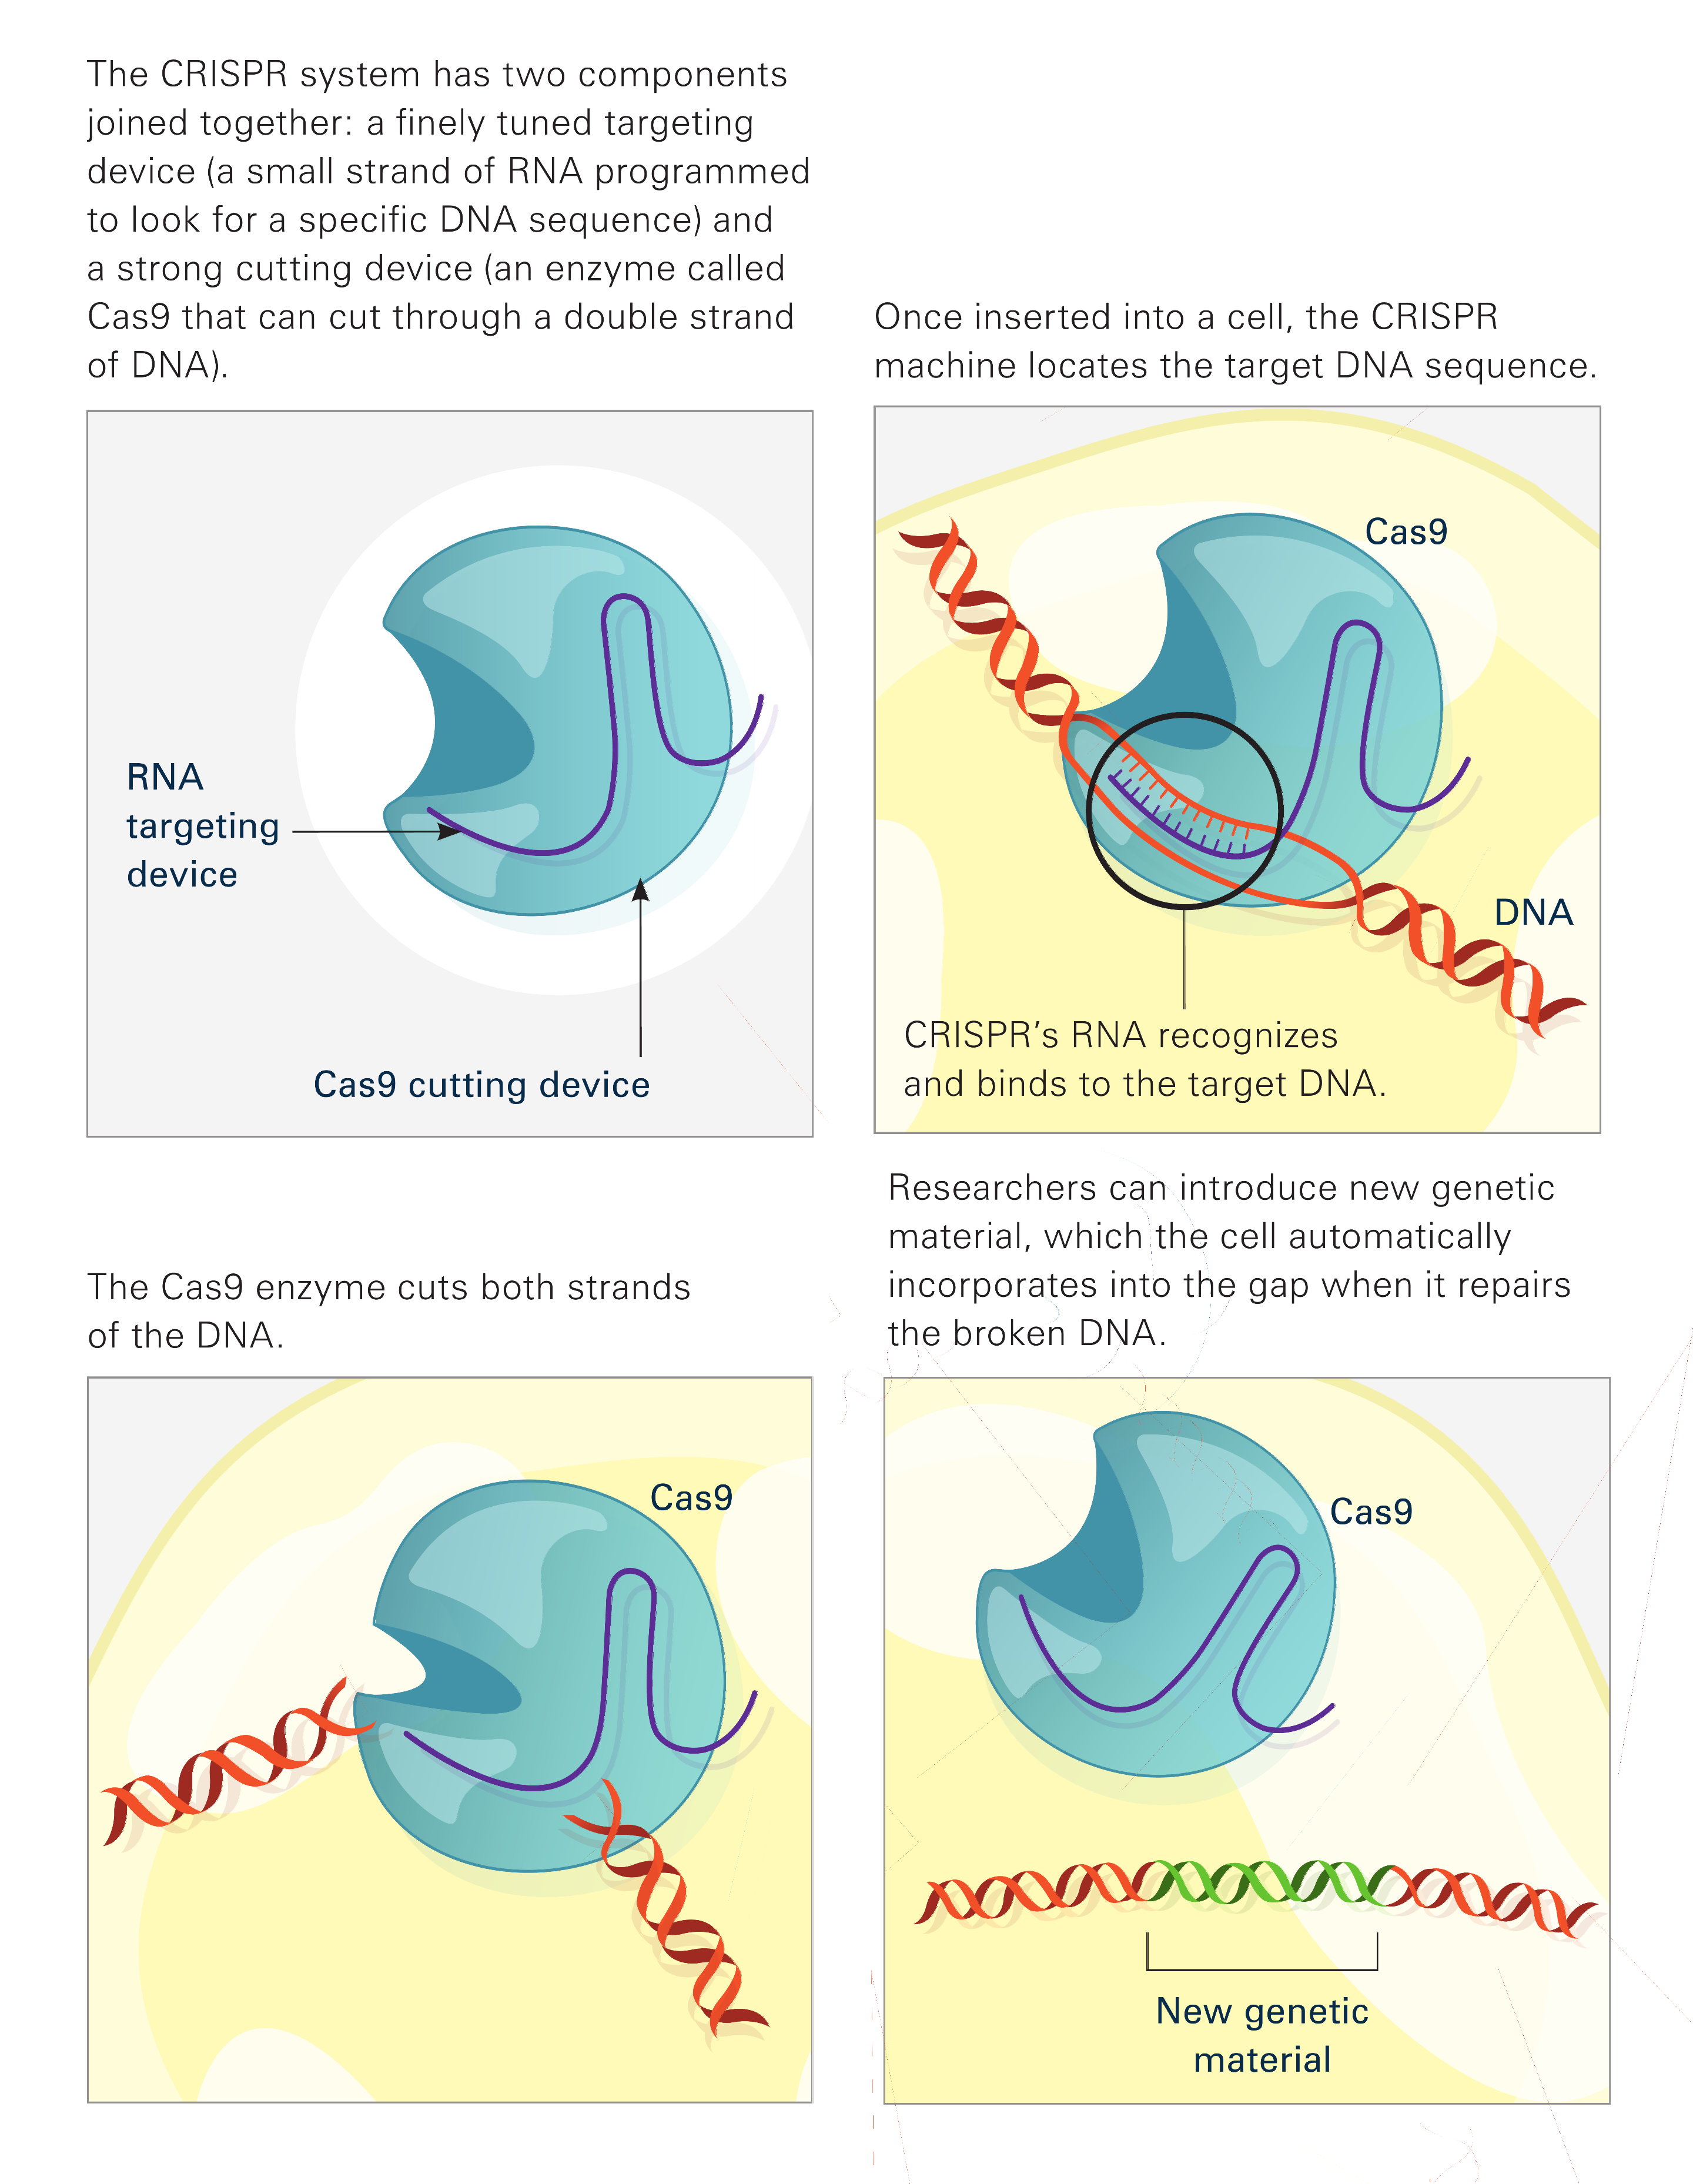
\includegraphics[width=0.85\linewidth]{figs/crispr_guide.png}
      \end{center}
    \end{column}
  \end{columns}
\end{frame}

% ------------------------------------------------------------------------------
\begin{frame}{1.3 The DepMap Project}
  \textbf{The Cancer Dependency Map (DepMap):}
  \begin{itemize}
    \item A large-scale resource identifying essential genes for tumor survival
          using genome-wide CRISPR knockout screens.
    \item Integrates multi-omics: copy number, gene expression, mutations, etc.
    \item Public portal: \href{https://depmap.org/portal/}{depmap.org/portal}
    \item dbGaP: \href{https://www.ncbi.nlm.nih.gov/projects/gap/cgi-bin/study.cgi?study_id=phs003444.v2.p1}{phs003444.v2.p1}
  \end{itemize}

  \vspace{0.3cm}
  \textbf{Why DepMap Matters:}
  \begin{itemize}
    \item Systematic “dependency” data across hundreds of cancer cell lines.
    \item Fuels precision oncology by linking genomic features to gene essentialities.
  \end{itemize}

  \vspace{0.2cm}
  \textbf{Note on ModelID:}
  \begin{itemize}
    \item Each DepMap cell line is assigned a unique \texttt{ModelID}.
    \item Ensures consistent referencing across CRISPR effect, dependency, CN, and expression data.
  \end{itemize}
\end{frame}

% ------------------------------------------------------------------------------
\begin{frame}{1.4 Key Score Definitions (CERES, Chronos, etc.)}
  \textbf{CERES Scores} (\textit{Main metric used in DepMap})
  \begin{itemize}
    \item Corrects for copy-number effects in CRISPR-Cas9 screens.
    \item Scale: Negative = essential, near 0 = non-essential.
    \item Large negative scores imply strong depletion (i.e., gene knockout is detrimental).
  \end{itemize}
  \vspace{0.3em}

  \textbf{Chronos Scores} (\textit{Alternative model to CERES})
  \begin{itemize}
    \item An alternative model that refines gene fitness effects over time.
    \item Often yields a heavier tail for highly essential genes.
    \item Generally correlates with CERES but can differ for common essentials.
  \end{itemize}
  \vspace{0.3em}

  \textbf{Dependency Probability} (\textit{Likelihood-based ranking of gene essentiality})
  \begin{itemize}
    \item Interpreted as the likelihood a gene is essential \& helps identify context-dependent vulnerabilities.
    \item Ranges from 0 (not dependent) to 1 (strongly dependent).
  \end{itemize}
  \vspace{0.3em}

  \textbf{Gene Expression} (\textit{mRNA abundance \& dependency correlation})
  \begin{itemize}
    \item Typically measured in log2(TPM+1).
    \item High expression can correlate with “oncogene addiction,” 
          but not always a direct proxy for essentiality.
  \end{itemize}
\end{frame}


% ------------------------------------------------------------------------------
\begin{frame}{1.5 Schematic of the CERES Model}
\begin{center}
  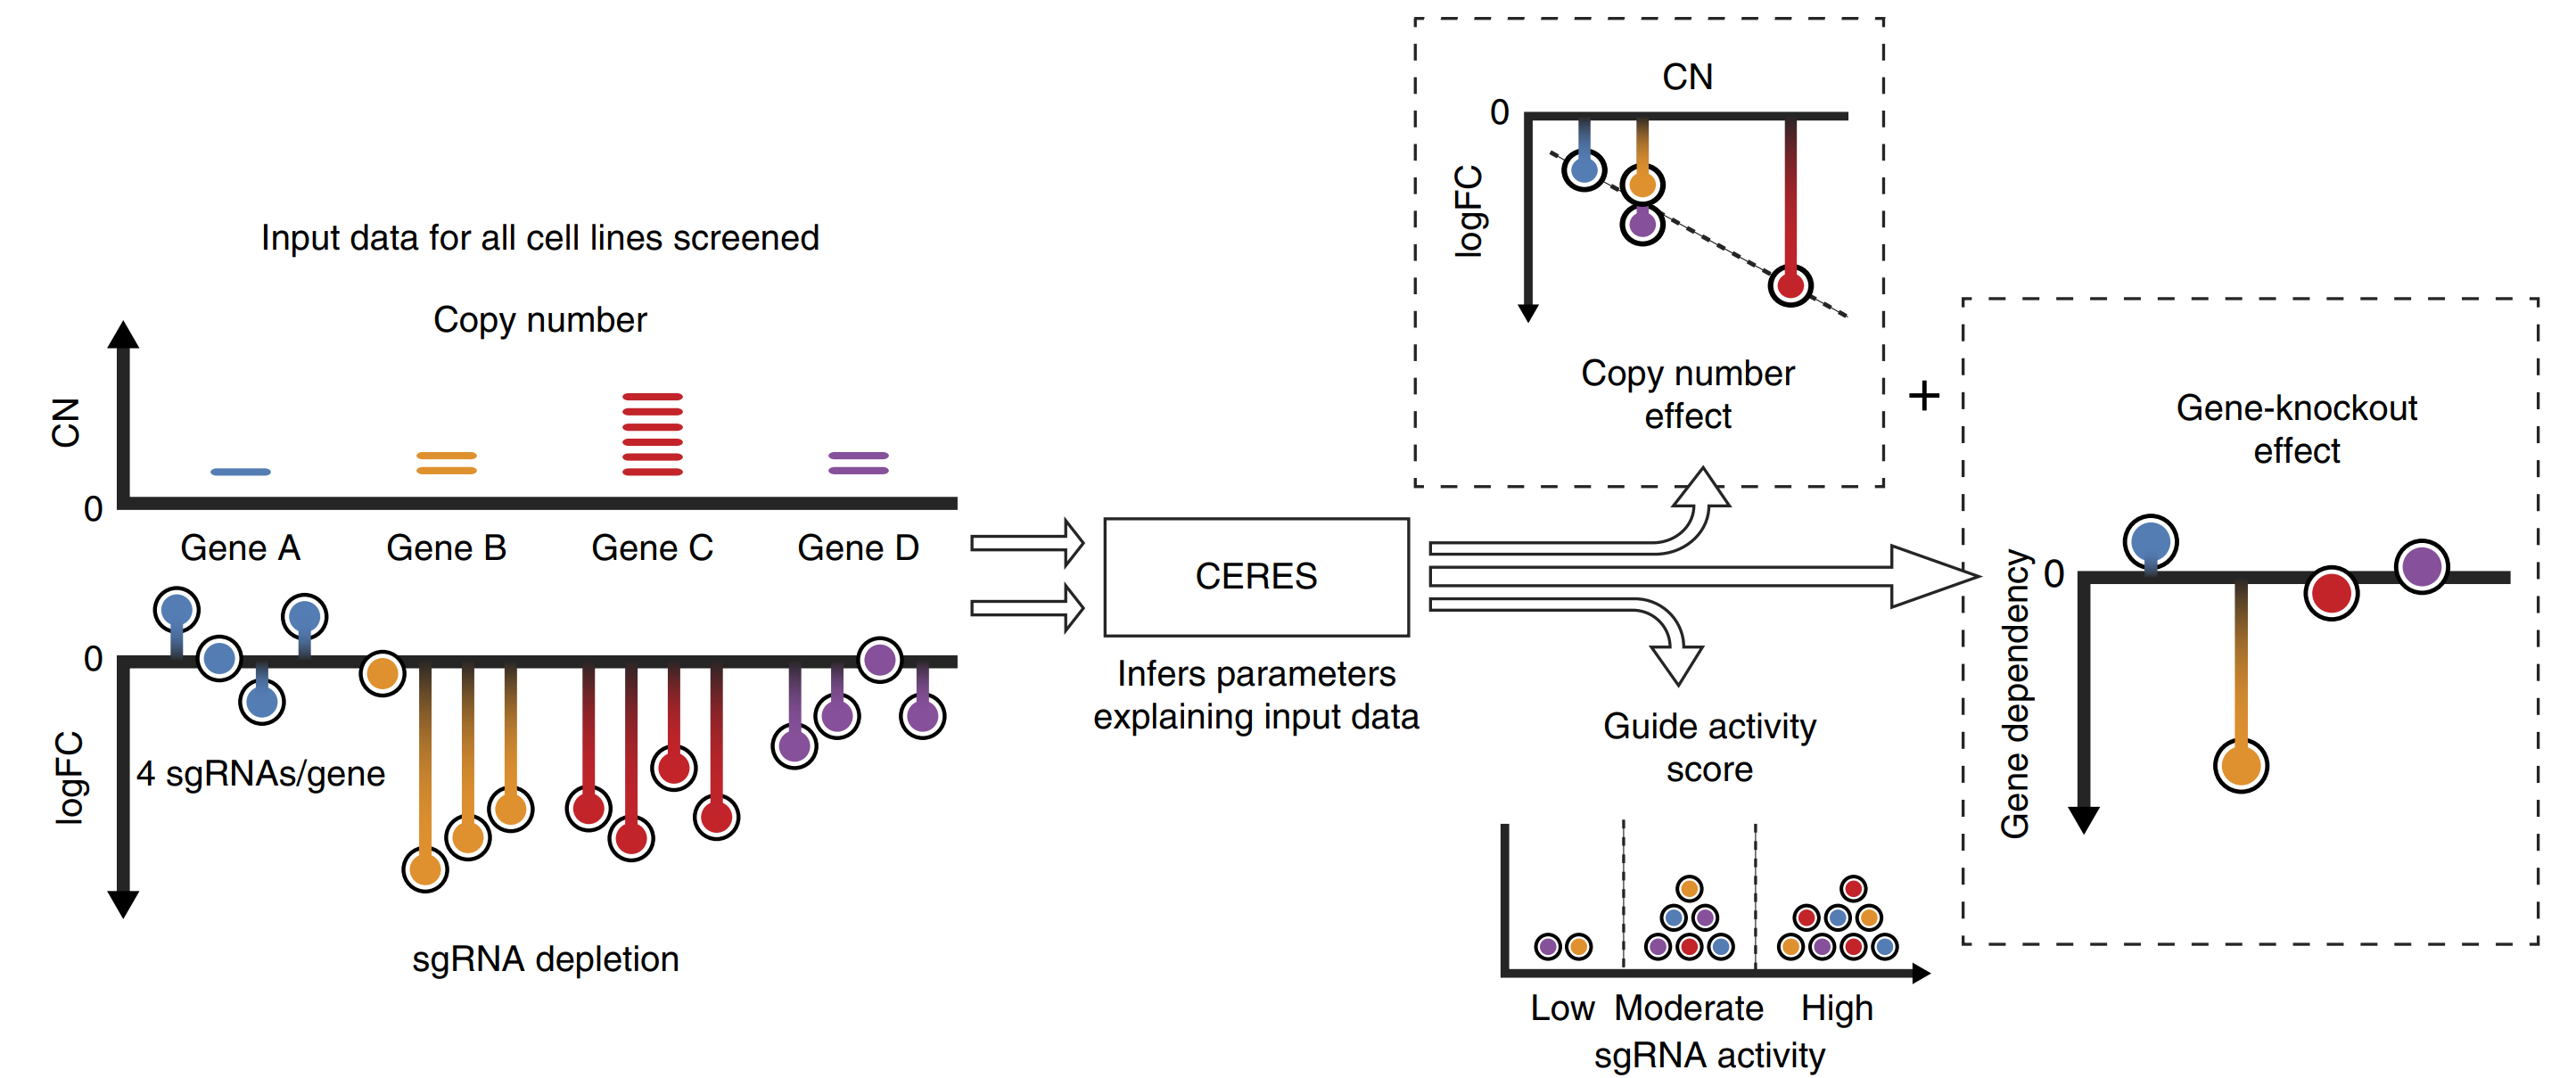
\includegraphics[width=1\linewidth]{figs/CERES-computational-model.png}
\end{center}

\footnotesize
\textbf{Figure:} Schematic of the CERES computational model.
As input, CERES takes sgRNA-depletion and copy number data for all cell lines screened. During the inference procedure, CERES models the depletion values as a sum of gene-knockout and copy number effects, multiplied by a guide activity score parameter. It infers the parameters (copy-number effect, guide efficiency, etc.) that best explain the observed CRISPR depletion data (maximum-likelihood of the observed data). 

\vspace{0.2em}
\textit{Source:} 
\href{https://doi.org/10.1038/ng.3984}{Meyers \emph{et al.}, \textit{Nature Genetics}, 2017.}
\end{frame}

% ------------------------------------------------------------------------------
\begin{frame}{Follow Along with the Tutorial}
  \textbf{Google Colab Notebook:}
  \begin{itemize}
    \item We have an interactive Jupyter/Colab notebook that walks through the data loading,
          merging, EDA, and modeling steps.
    \item \textit{Link:}
      \href{https://colab.research.google.com/drive/12B8lswKoV_u2tAzg_mTVrqM9VQvqinOg}{\textbf{\underline{Colab Notebook}}}
    \item Download or open directly to run each cell and replicate the results.
  \end{itemize}
\end{frame}


% ==============================================================================
\section{2. Data Preprocessing \& Overview}
% ==============================================================================

% ------------------------------------------------------------------------------
\begin{frame}{2.1 Data Preprocessing Workflow}
  \textbf{Goals:} 
  \begin{itemize}
    \item Subset large DepMap files to genes of interest.
    \item Standardize column names (e.g., \texttt{ModelID}).
    \item Prepare consistent CSV files for downstream EDA and modeling.
  \end{itemize}

  \vspace{0.3cm}
  \textbf{Script: \texttt{filter-preprocess-data.py}} (\href{https://github.com/ChestnutKurisu/MED263_Final_Project_WI25/blob/main/preprocessing-pipeline/filter-preprocess-data.py}{GitHub Link})
  \begin{itemize}
    \item \textbf{Select Genes:} 
      \begin{itemize}
        \item Curated list of core cancer genes (e.g., \texttt{TP53}, \texttt{EGFR}, \texttt{KRAS}, \texttt{BRCA1}, etc.).
      \end{itemize}
    \item \textbf{Chunk Reading:}
      \begin{itemize}
        \item DepMap CSVs can be hundreds of MBs.
        \item Reads in chunks of 5000 rows, concatenates selected columns.
      \end{itemize}
    \item \textbf{Outputs:}
      \begin{itemize}
        \item \texttt{CRISPRGeneEffect.csv}, \texttt{CRISPRGeneDependency.csv}
        \item \texttt{OmicsCNGene.csv}, \texttt{OmicsSomaticMutationsMatrixDamaging.csv}
        \item \texttt{OmicsExpressionProteinCodingGenesTPMLogp1.csv} (plus stranded version)
      \end{itemize}
  \end{itemize}

\end{frame}

% ------------------------------------------------------------------------------
\begin{frame}{2.2 Preprocessing Steps}
  \textbf{Key Highlights:}
  \begin{enumerate}
    \item \textbf{Fix Headers:} 
      \begin{itemize}
        \item The script checks for blank or unnamed columns and renames them to \texttt{"ModelID"}.
      \end{itemize}
    \item \textbf{Filter by Genes:} 
      \begin{itemize}
        \item Retains only columns matching the user-provided list (e.g., \texttt{EGFR}, \texttt{BRCA1}, etc.).
      \end{itemize}
    \item \textbf{Save Cleaned CSVs:} 
      \begin{itemize}
        \item Each subset is saved in an output directory (e.g., \texttt{DepMap-preprocessed/}).
      \end{itemize}
  \end{enumerate}

  \vspace{0.3cm}
  \textbf{Motivation:}
  \begin{itemize}
    \item Reduces file size, speeds up analysis.
    \item Ensures consistent \texttt{ModelID} merges across multiple omics layers.
  \end{itemize}
\end{frame}

% ==============================================================================
\section{3. Data Loading \& EDA}
% ==============================================================================

% ------------------------------------------------------------------------------
\begin{frame}{3.1 Data Loading Overview}
  \textbf{Files merged on \texttt{ModelID}:}
  \begin{itemize}
    \item \texttt{CRISPRGeneEffect.csv} (Chronos-corrected effect scores)
    \item \texttt{CRISPRGeneDependency.csv} (Dependency probabilities)
    \item \texttt{OmicsCNGene.csv}, \texttt{OmicsSomaticMutationsMatrixDamaging.csv}
    \item \texttt{OmicsExpressionProteinCodingGenesTPMLogp1.csv}
    \item \texttt{Model.csv} for lineage \& metadata
  \end{itemize}
  \vspace{0.3cm}
  \textbf{Cleaning Steps:}
  \begin{enumerate}
    \item Renamed columns to \texttt{GENE\_eff}, \texttt{GENE\_dep}, \texttt{GENE\_CN}, \texttt{GENE\_mut}, \texttt{GENE\_expr}.
    \item Filtered missing or inconsistent rows.
    \item Merged into a final \texttt{merged\_df}.
  \end{enumerate}
\end{frame}

% ------------------------------------------------------------------------------
\begin{frame}{3.2.1 ARID1A: Selected Gene of Interest}
  \textbf{ARID1A Overview:}
  \begin{itemize}
    \item \textbf{Gene Name:} AT-Rich Interaction Domain 1A
    \item \textbf{Function:} Core component of the SWI/SNF chromatin-remodeling complex.
    \item \textbf{Clinical Relevance:} 
      \begin{itemize}
        \item Frequently mutated in ovarian clear-cell carcinoma, endometrial carcinoma.
        \item Functions primarily as a tumor-suppressor gene.
      \end{itemize}
    \item \textbf{OMIM Link:} \href{https://omim.org/entry/603024}{OMIM ARID1A (603024)}
  \end{itemize}

  \vspace{0.3cm}
  \textbf{Why ARID1A?}
  \begin{itemize}
    \item Mutations can lead to partial or complete loss-of-function in tumor suppression.
    \item DepMap reveals variability in ARID1A essentiality across different cell lines.
    \item ARID1A is a \textbf{tumor suppressor}, so loss-of-function mutations 
can promote tumorigenesis. In CRISPR screens, ARID1A-knockout often shows weaker effects in lines 
already harboring a damaging mutation.
  \end{itemize}
\end{frame}

% ------------------------------------------------------------------------------
\begin{frame}{3.2.2 KRAS: Selected Gene of Interest}
  \textbf{KRAS (Kirsten Rat Sarcoma Viral Oncogene Homolog)}
  \begin{itemize}
    \item One of the most commonly mutated \textbf{proto-oncogenes} in human cancer.
    \item Encodes a GTPase regulating cell proliferation, differentiation, and survival.
    \item \textbf{Activating mutations} often lock KRAS in a GTP-bound “active” state.
    \item Prevalent in \textbf{pancreatic}, \textbf{colorectal}, and \textbf{lung} cancers,
      driving oncogenic signaling (e.g., MAPK-ERK).
    \item \textbf{OMIM Link:} \href{https://omim.org/entry/190070}{OMIM KRAS (190070)}
  \end{itemize}

  \vspace{0.3cm}
  \textbf{Clinical \& Therapeutic Relevance:}
  \begin{itemize}
    \item Major driver of tumor initiation and progression in many cancer types.
    \item Under active investigation for targeted therapies (e.g., KRAS(G12C) inhibitors).
    \item Mutations can also be associated with certain developmental syndromes (e.g. Noonan).
    \item KRAS is an \textbf{oncogene}; its mutations enhance cell growth and proliferation. CRISPR knockout yields strongly negative scores in cell lines highly dependent on KRAS signaling.
  \end{itemize}
\end{frame}

% ------------------------------------------------------------------------------
\begin{frame}{3.3 Exploratory Data Analysis (EDA)}
  \textbf{Initial Checks:}
  \begin{itemize}
    \item Summary statistics for effect \& dependency scores.
    \item Gene expression distributions (log2(TPM+1)).
    \item Mutation frequencies: \texttt{ARID1A}: $\sim$10\% mutated lines (total 118/1178);
          \newline e.g., \texttt{ARID1A\_mut} distribution: 
            \texttt{0 = 1060, 1 = 68, 2 = 50}.
  \end{itemize}

  \vspace{0.2cm}
  \textbf{Pitfalls:}
  \begin{itemize}
    \item Some lineages with very few samples \(\rightarrow\) less statistical power.
    \item Expression outliers from highly amplified genes.
    \item Non-normal score distributions \(\rightarrow\) Mann--Whitney U or other nonparametric tests.
  \end{itemize}
\end{frame}

% ------------------------------------------------------------------------------
\begin{frame}{3.4 ARID1A Effect Score Distribution}
  \begin{itemize}
    \item Negative Chronos effect implies higher essentiality.
    \item ARID1A has mean score \(\approx -0.236\), a small fraction of lines $< -1$.
  \end{itemize}
  \vspace{0.2cm}
  \begin{center}
      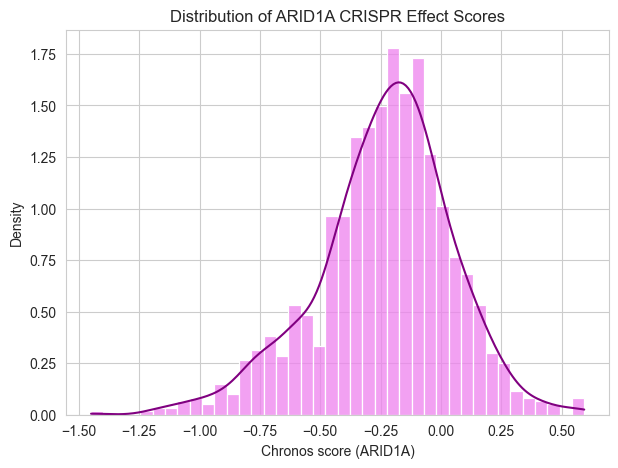
\includegraphics[width=0.5\linewidth]{figs/arid1a_effect_histogram.png}
  \end{center}

  \vspace{0.2cm}
  \textbf{Interpretation:}
  \begin{itemize}
    \item Heterogeneous essentiality distribution: many lines near mild essentiality or neutral.
    \item Strongly negative tail indicates a subset highly dependent on ARID1A.
  \end{itemize}
\end{frame}

% ------------------------------------------------------------------------------
\begin{frame}{3.5 KRAS: Lineage-Specific Effect Scores}
  \begin{itemize}
    \item \textbf{Pancreatic} cell lines show the most negative median KRAS effect 
          ($\approx -1.76$), consistent with strong KRAS dependency.
    \item \textbf{Bowel (colorectal)} lines also rank highly in negative KRAS scores, 
          aligning with frequent KRAS mutations in colorectal cancer.
    \item \textbf{Less negative medians} (e.g., Kidney) suggest lower KRAS dependence, 
          possibly due to alternate oncogenic drivers.
    \item Overall, these data underscore \emph{lineage-specific KRAS essentiality}, 
          matching the known biology that KRAS is a critical driver in pancreatic 
          and colorectal tumors but may be less central in other tissues.
  \end{itemize}
    \begin{center}
      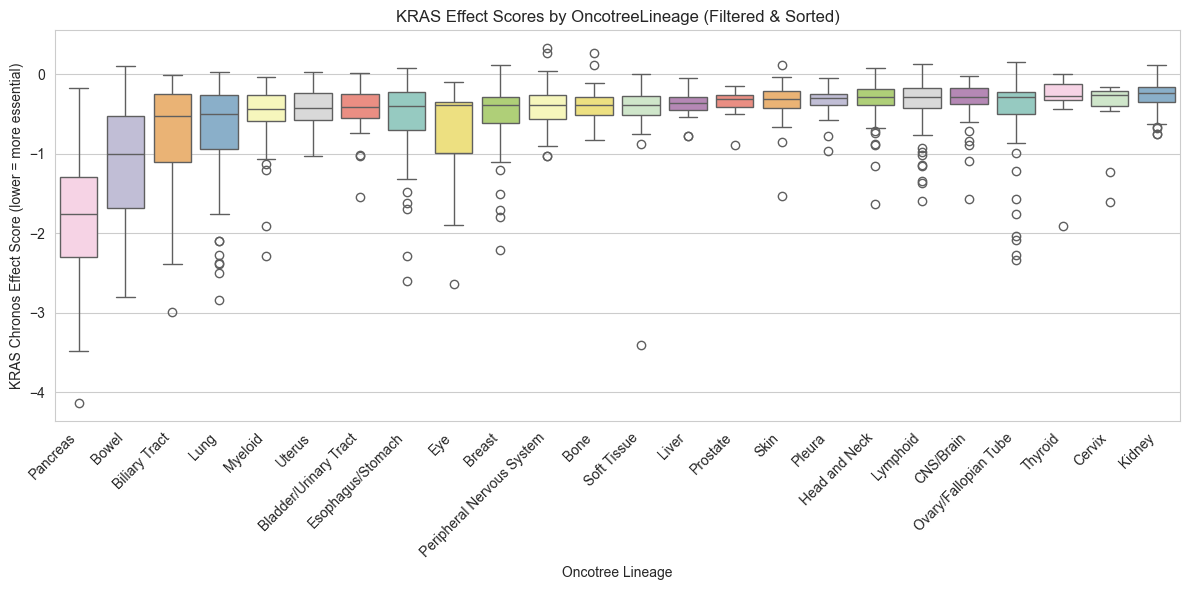
\includegraphics[width=0.74\linewidth]{figs/kras_lineage_boxplot.png}
    \end{center}
\end{frame}

% ==============================================================================
\section{4. Dimensionality Reduction}
% ==============================================================================

% ------------------------------------------------------------------------------
\begin{frame}{4.1 PCA Projection}
  \textbf{Goal:} Summarize thousands of features into a few principal components.
  \begin{itemize}
    \item PC1 + PC2 often explain $< 20\%$ of total variance.
    \item Tissue-specific clustering not strongly observed.
  \end{itemize}
  \vspace{0.2cm}
  \begin{center}
    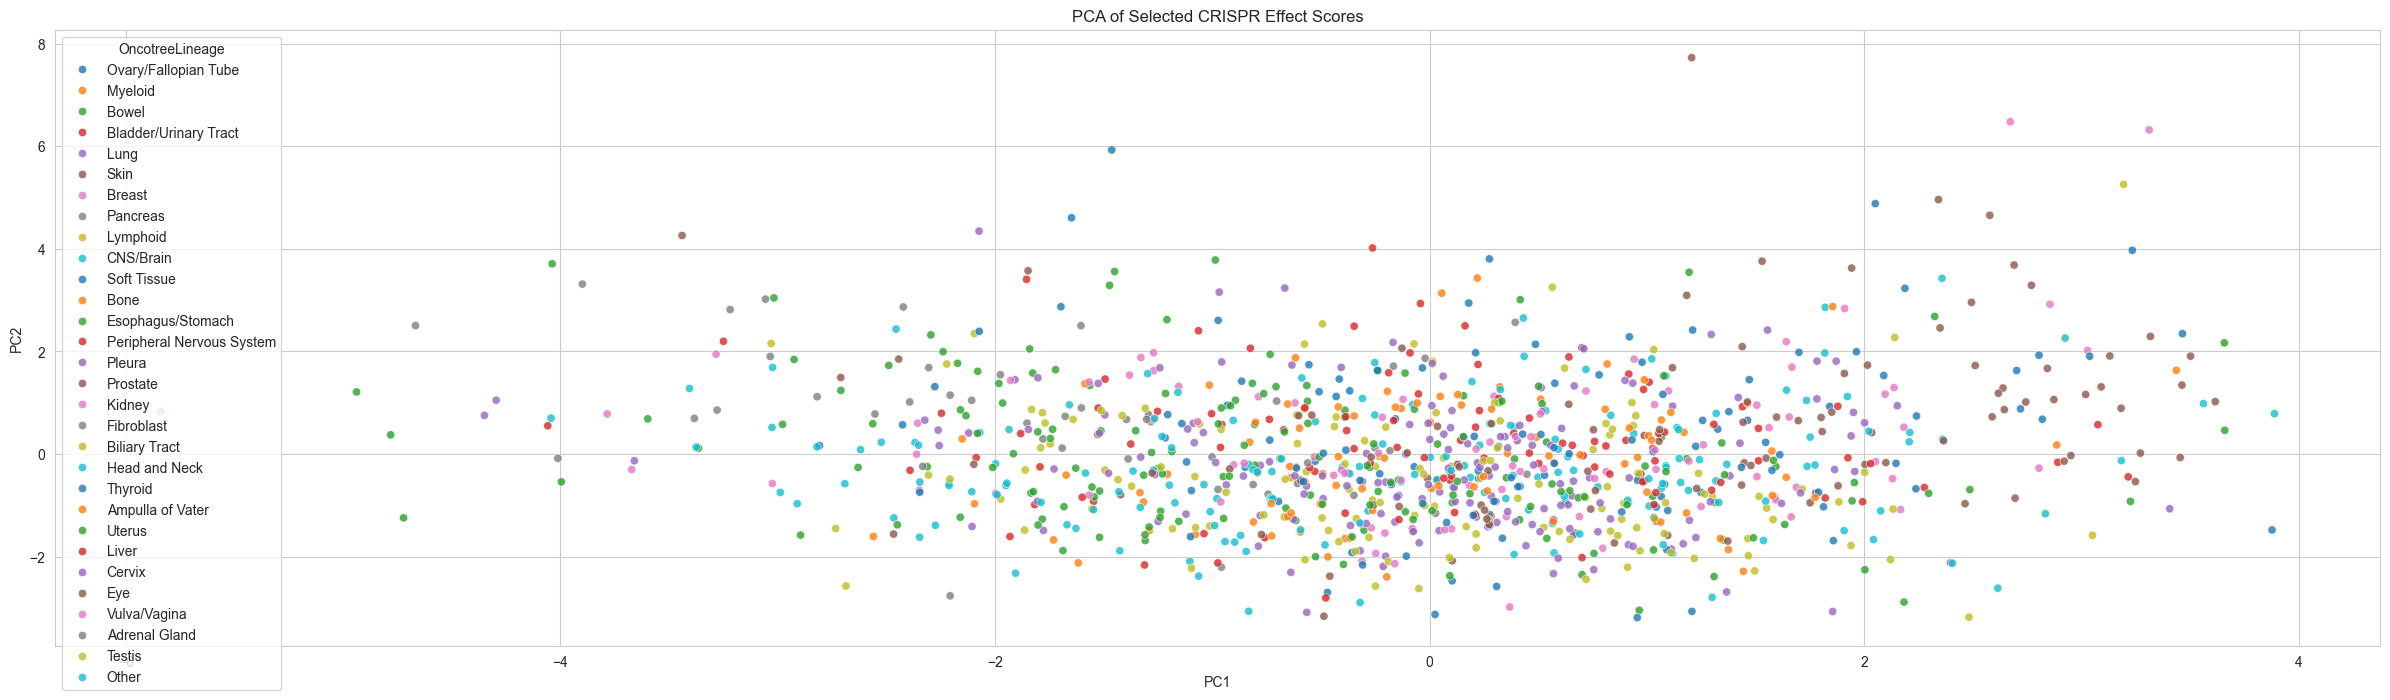
\includegraphics[width=1\linewidth]{figs/pca_projection.png}
  \end{center}
\end{frame}

% ------------------------------------------------------------------------------
\begin{frame}{4.2 UMAP Results}
  \begin{itemize}
    \item \textbf{UMAP} better preserves local distances; partial lineage clustering but still overlapping.
    \item Suggests that CRISPR effect scores alone do not strictly separate lineages in 2D.
  \end{itemize}
  \vspace{0.3cm}
  \begin{center}
    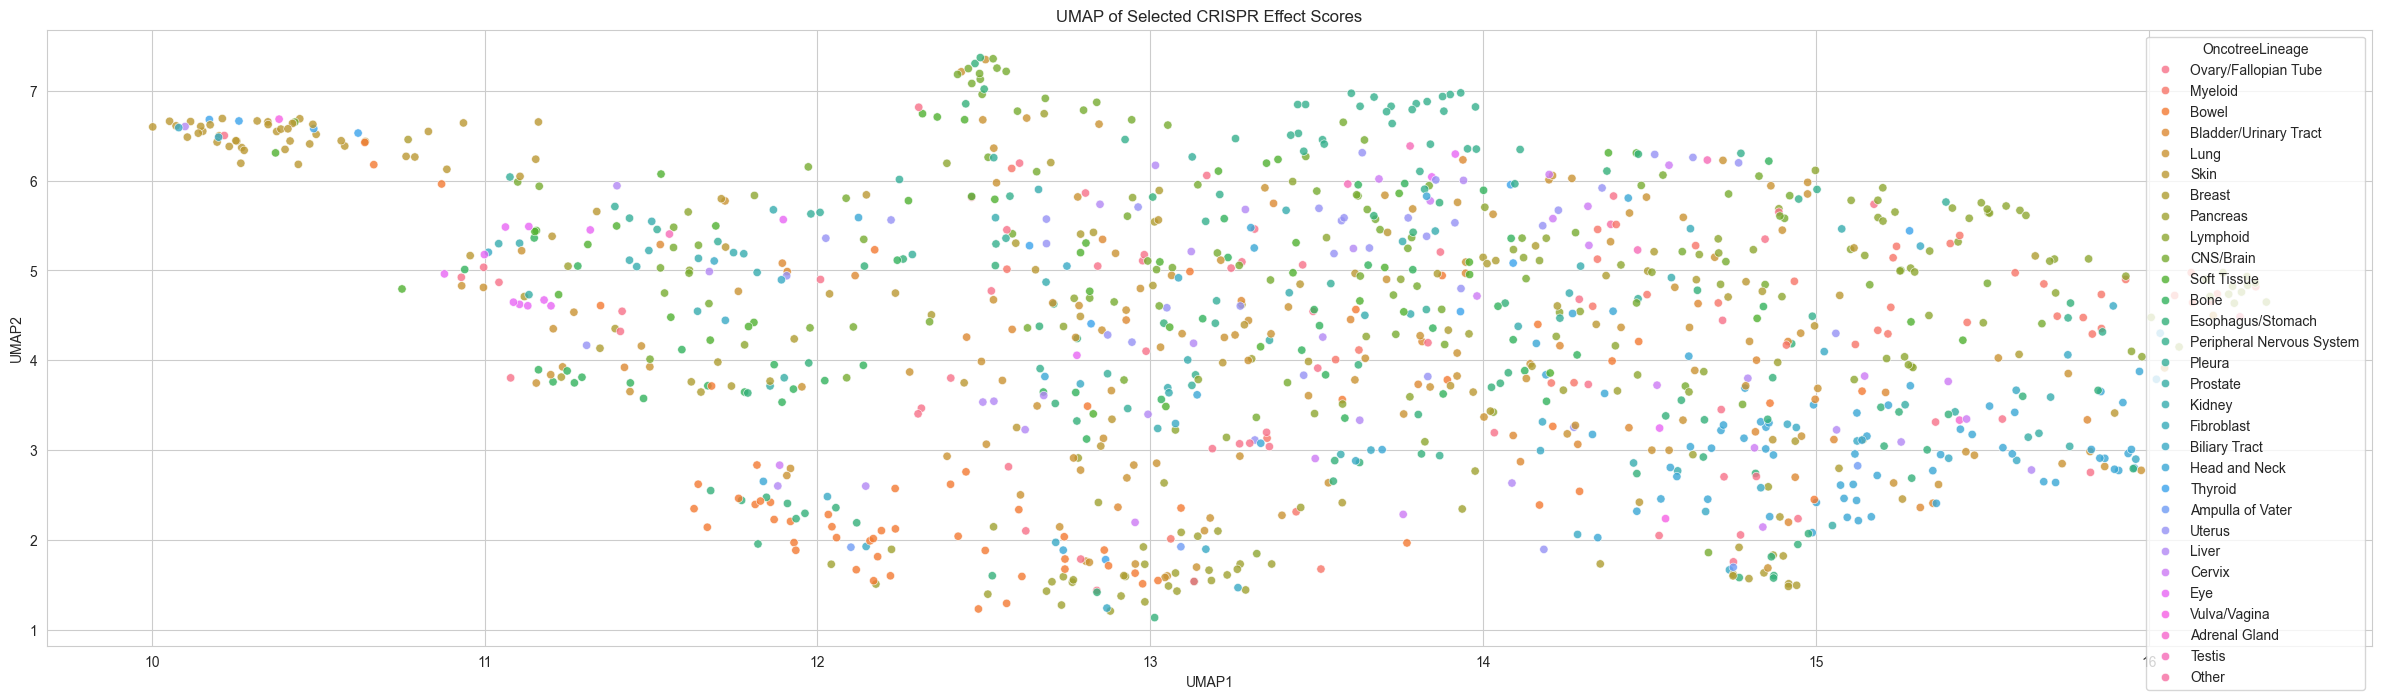
\includegraphics[width=1\linewidth]{figs/umap_projection.png}
  \end{center}
\end{frame}

% ==============================================================================
\section{5. Statistical Tests \& Multi-Omics Associations}
% ==============================================================================

% ------------------------------------------------------------------------------
\begin{frame}{5.1 Mann--Whitney U: ARID1A Mutant vs. WT}
  \textbf{Hypothesis:} ARID1A knockout has different effects in mutant vs. wild-type lines.
  \begin{itemize}
    \item p-value \(\approx 9.17 \times 10^{-11}\) \(\to\) highly significant difference.
    \item Mutant lines \(\to\) less negative (knockout has weaker impact if gene is already partly inactivated).
    \item WT lines \(\to\) more negative effect (fully functional ARID1A crucial).
  \end{itemize}

  \vspace{0.3cm}
  \begin{center}
    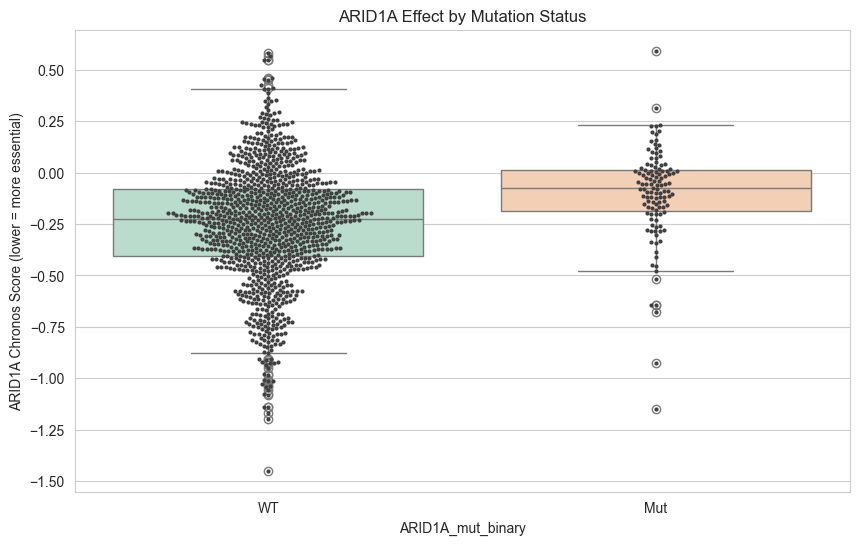
\includegraphics[width=0.7\linewidth]{figs/arid1a_mw_boxplot.png}
  \end{center}
\end{frame}

% ------------------------------------------------------------------------------
\begin{frame}{5.2 ARID1A Effect vs. Dependency \& Correlation Matrix}
  \textbf{Correlation Matrix (ARID1A\_eff, \_dep, \_expr, \_mut, etc.)}
  \begin{itemize}
    \item \(\mathrm{Corr}(\text{ARID1A\_eff}, \text{ARID1A\_dep}) \approx -0.92\).
    \item \(\mathrm{Corr}(\text{ARID1A\_eff}, \text{ARID1A\_expr})\) weaker, near -0.10.
  \end{itemize}

  \begin{center}
    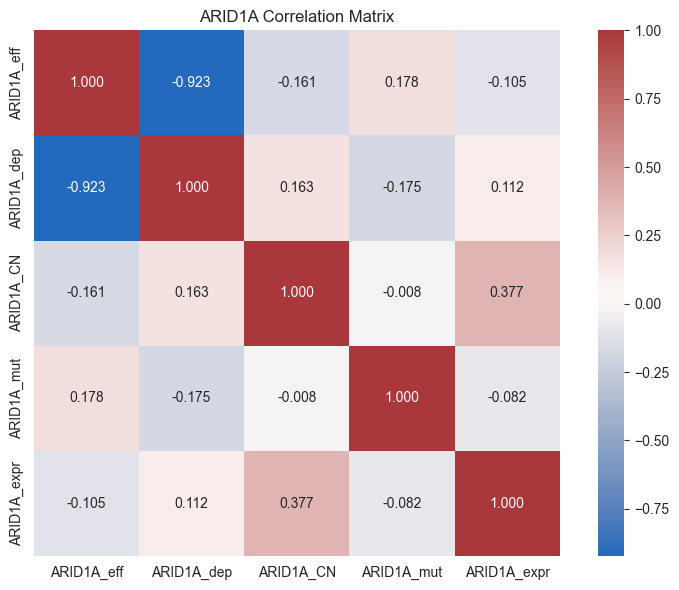
\includegraphics[width=0.42\linewidth]{figs/arid1a_correlation_matrix.png}
  \end{center}

  \textbf{Interpretation:}  
  \begin{itemize}
    \item \texttt{ARID1A\_dep} is inversely correlated with \texttt{ARID1A\_eff} (more negative = higher dependency).
    \item Expression alone does not strongly predict essentiality for ARID1A.
  \end{itemize}
\end{frame}

% ------------------------------------------------------------------------------
\begin{frame}{5.3 ARID1A Effect vs. Dependency}
  \textbf{Chronos effect score vs. dependency probability}
  \begin{itemize}
    \item Often strongly (negatively) correlated: more negative effect $\to$ higher probability of essentiality.
    \item \textbf{Non-linear fit}: a tanh or logistic curve can model the saturation at extremes.
  \end{itemize}

  \vspace{0.05cm}
  \textbf{Plot:} $\mathrm{ARID1A}_{\mathrm{dep}} \approx 0.4996\tanh(-3.6348\,\mathrm{ARID1A}_{\mathrm{eff}} - 1.5996) + 0.4838$.
    \begin{center}
      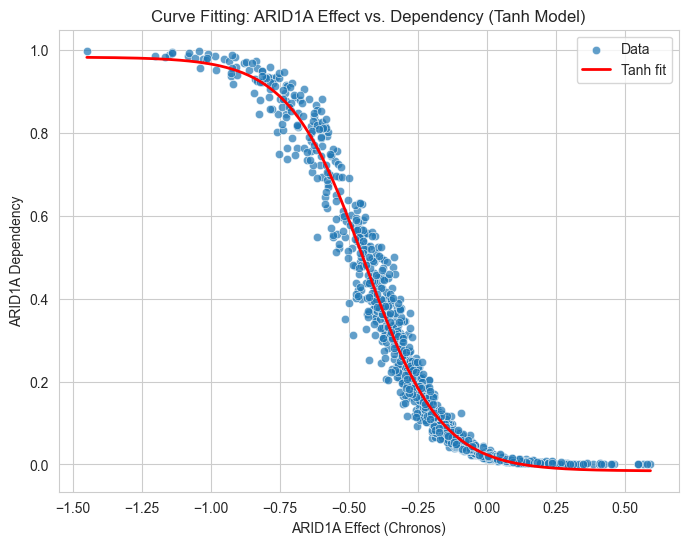
\includegraphics[width=0.6\linewidth]{figs/arid1a_scatter_tanh.png}
    \end{center}

  \vspace{0.05cm}
  \textbf{Interpretation:} 
  \begin{itemize}
    \item Scores $<-1 \to$ near-max dependency.
    \item Scores around $>0 \to$ near-min dependency.
  \end{itemize}
\end{frame}

% ==============================================================================
\section{6. Random Forest \& Multi-Omics Integration}
% ==============================================================================

% ------------------------------------------------------------------------------ 

\begin{frame}{6.1 Single-Gene Random Forest: KRAS Dependency}
  \textbf{Goal:} Predict \(\texttt{KRAS\_dep} \in [0, 1]\) using expression, copy number, mutation data,
  and metadata (Oncotree lineage, etc.).

  \vspace{0.3cm}
  \textbf{Model:} \(\texttt{RandomForestRegressor}\) with 100 trees, trained on an 80/20 split of 1178 samples.

  \vspace{0.2cm}
  \textbf{Results:}
  \begin{itemize}
    \item \(R^2 \approx 0.2637\) on the held-out test set.
    \item MSE \(\approx 0.078\).
    \item \textbf{Top Features}:
      \begin{itemize}
        \item \(\texttt{KRAS\_CN}\) (copy number) 
        \item \(\texttt{OncotreeLineage\_Pancreas}\)
        \item \(\texttt{OncotreeLineage\_Bowel}\)
        \item \(\texttt{MET\_expr}, \texttt{EGFR\_CN}, \texttt{PTEN\_CN}\), etc.
      \end{itemize}
  \end{itemize}

  \vspace{0.1cm}
  \textbf{Interpretation:}
  \begin{itemize}
    \item Amplifications/deletions of \texttt{KRAS} drive dependency strength.
    \item \textbf{Lineage} (pancreatic, colorectal) is crucial: known KRAS-addicted tumors.
    \item Additional CN changes (e.g. \texttt{EGFR}, \texttt{PTEN}) modulate KRAS reliance.
  \end{itemize}
\end{frame}

% ------------------------------------------------------------------------------ 
\begin{frame}{6.2 Multi-Gene Regression with Random Forest}
  \textbf{Approach:} MultiOutput Random Forest to predict multiple gene dependencies simultaneously from the same multi-omics + metadata feature set.

  \begin{itemize}
    \item Retained genes with \(\sigma(\text{dep}) \geq 0.25\).
    \item Trained on all lines with non-missing data (\(n \approx 1178\)).
    \item Evaluate each gene's \(R^2\) and MSE individually.
  \end{itemize}

  \vspace{0.3cm}
  \textbf{Findings:}
  \begin{itemize}
    \item \texttt{CTNNB1\_dep}: highest \(R^2 \approx 0.58\).
    \item \texttt{CDK6\_dep}: \(R^2 \approx 0.46\).
    \item \texttt{KRAS\_dep}: \(R^2 \approx 0.26\).
    \item Tumor suppressors like \texttt{BRCA1}, \texttt{ARID1A} show lower predictability (\(R^2 \approx 0.04\text{--}0.06\)).
  \end{itemize}

  \textbf{Interpretation:} 
  \begin{itemize}
    \item Genes central to known oncogenic pathways (e.g., \(\beta\)-catenin/Wnt) are more systematically predicted by lineage and multi-omics signals.
    \item Tumor-suppressor essentialities can be more context-dependent or confounded by partial/inactivating mutations.
  \end{itemize}
\end{frame}

% ------------------------------------------------------------------------------ 
\begin{frame}{6.3 Unsupervised Clustering of Cell Lines}
  \textbf{Method:}
  \begin{itemize}
    \item Used PCA on expression and CN features (scaled), then KMeans \((k=5)\).
    \item Clusters do not perfectly match single lineages; some groups are mixed.
  \end{itemize}

  \begin{columns}
    \begin{column}{0.5\linewidth}
      \begin{itemize}
        \item \textbf{Cluster 0}: Lymphoid, Skin, Myeloid
        \item \textbf{Cluster 1}: Lung, CNS/Brain, Uterus
        \item \textbf{Cluster 2}: CNS/Brain, Lung, Bone
        \item \textbf{Cluster 3}: Bowel-dominant cluster
        \item \textbf{Cluster 4}: Head/Neck, Stomach, Pancreas
      \end{itemize}
    \end{column}
    \begin{column}{0.5\linewidth}
      \begin{center}
      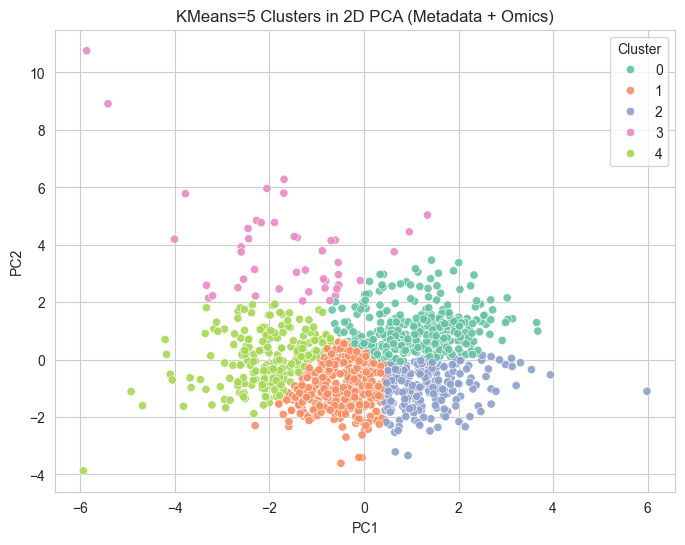
\includegraphics[width=0.85\linewidth]{figs/kmeans_pca_plot.png}
      \end{center}
    \end{column}
  \end{columns}

  \vspace{0.3cm}
  \textbf{Takeaway:} Some lineages cluster together, but there's overlap. 
  Multi-omics signals can partition certain subtypes (e.g., Bowel, Head/Neck).
\end{frame}

% ==============================================================================
\section{7. Conclusions \& Next Steps}
% ==============================================================================

% ------------------------------------------------------------------------------
\begin{frame}{7. Conclusions \& Future Directions}
  \begin{block}{Key Takeaways}
    \begin{itemize}
      \item \textbf{ARID1A} shows context-dependent essentiality:
        \begin{itemize}
          \item Mutant lines have weaker knockout effects.
          \item Mann--Whitney p-value $\sim 9.17\times 10^{-11}$.
        \end{itemize}
      \item \textbf{KRAS dependency} strongly linked to lineage (pancreatic, bowel)
            and copy-number variations (\(\texttt{KRAS\_CN}\)).
            Single-gene RF yields \(R^2 \approx 0.26\).
      \item \textbf{Multi-gene RF} reveals \texttt{CTNNB1}, \texttt{CDK6} are more predictable
            (\(R^2>0.45\)), whereas \texttt{BRCA1}, \texttt{ARID1A} remain difficult to predict (\(R^2<0.10\)).
    \end{itemize}
  \end{block}

  \begin{block}{Next Steps}
    \begin{itemize}
      \item Further refine multi-omics (proteomics, epigenetics, drug-response data) for more accurate essentiality predictions.
      \item Investigate advanced ML (deep neural networks, ensemble methods) for gene dependencies.
    \end{itemize}
  \end{block}
\end{frame}

% ==============================================================================
\section{8. CRISPR in Practice: Current State \& Applications}
% ==============================================================================

% ------------------------------------------------------------------------------
\begin{frame}{8.1 CRISPR in Cancer: Clinical Trials \& Immunotherapy}
  \textbf{CRISPR-Based Cell Therapies:}
  \begin{itemize}
    \item \textit{Ex vivo} approach: Editing T cells (e.g., knocking out \textbf{PD-1}, TCR genes)
          and re-infusing them to enhance tumor targeting.
    \item Early-phase \textbf{CRISPR-CAR T-cell} trials in blood cancers show feasibility \& safety.
    \item Allogeneic (off-the-shelf) CAR T-cells leverage multiplex gene edits to avoid graft-vs-host disease.
  \end{itemize}

  \vspace{0.3em}
  \textbf{In Vivo Gene Editing:}
  \begin{itemize}
    \item Researchers exploring direct delivery (via gels, viral/lipid nanoparticles) to \textit{knock out}
          oncogenes \textit{in situ}, although still early-stage.
    \item Example: CRISPR gel targeting HPV E6/E7 in cervical lesions.
  \end{itemize}

  \vspace{0.3em}
  \textbf{Proof of Concept:}
  \begin{itemize}
    \item First CRISPR therapy (\emph{exa-cel}, for sickle cell) approved in 2023,
          heralding clinical acceptance of CRISPR-based treatments.
    \item Similar ex vivo editing strategies are now applied in oncology pipelines.
  \end{itemize}
\end{frame}

% ------------------------------------------------------------------------------
\begin{frame}{8.2 Base Editing, Prime Editing, \& Off-Target Mitigation}
  \textbf{Base Editing:}
  \begin{itemize}
    \item Creates precise point mutations (e.g. C-to-T) without a double-strand break.
    \item Enables complex “multi-gene” edits in T-cells, reducing large genomic rearrangements.
    \item Already entering clinical trials for T-ALL (quadruple-edited CAR T-cells).
  \end{itemize}

  \vspace{0.3em}
  \textbf{Prime Editing:}
  \begin{itemize}
    \item Uses a reverse transcriptase with Cas9 nickase to “search-and-replace” DNA sequences.
    \item Can theoretically fix a wide range of mutations \textit{in situ}.
    \item Currently lower efficiency than base editing, but active improvements are ongoing.
  \end{itemize}

  \vspace{0.3em}
  \textbf{Off-Target Effects \& Safety:}
  \begin{itemize}
    \item High-fidelity Cas9 variants and advanced guide design reduce unintended cuts.
    \item FDA/EMA approvals require robust off-target screening (e.g., GUIDE-seq) and long-term monitoring.
    \item \textit{Ex vivo} protocols further minimize immunogenic risk by removing Cas9 protein before infusion.
  \end{itemize}
\end{frame}

% ------------------------------------------------------------------------------
\begin{frame}{8.3 Ethical, Regulatory, \& Commercial Outlook}
  \textbf{Ethical \& Regulatory Considerations:}
  \begin{itemize}
    \item Worldwide prohibition on \textbf{germline} editing (heritable changes);
          clinical focus remains on \textbf{somatic} therapies.
    \item Regulators (FDA, EMA) demand thorough safety data:
          off-target analyses, immune response checks, post-trial surveillance.
    \item Affordability \& equitable access remain major concerns as gene-edited therapies
          tend toward high initial costs.
  \end{itemize}

  \vspace{0.3em}
  \textbf{Industry \& Future Directions:}
  \begin{itemize}
    \item Biotechs (CRISPR Therapeutics, Editas, Intellia, Beam) lead the push toward commercialization:
          ex vivo CAR T-cells, in vivo editing, base editing, prime editing.
    \item Ongoing wave of Phase I/II trials for solid \& hematologic cancers.
          Positive safety + efficacy could drive Phase III expansions.
    \item Integrating \textbf{multi-omics data} (like DepMap) will refine targeting strategies,
          enabling personalized CRISPR interventions.
  \end{itemize}
\end{frame}

% ==============================================================================
\begin{frame}[allowframebreaks]{References}
  \footnotesize
  \setlength{\parskip}{0pt}
  \begin{thebibliography}{99}

  % -- Original References --

  \bibitem{DepMapPortal}
    DepMap, Broad Institute. (2025).
    \emph{DepMap: The Cancer Dependency Map Project.} \href{https://depmap.org/portal/}{https://depmap.org/portal/}

  \bibitem{PMC10464129}
    Krill-Burger et al. (2023).
    \emph{Multi-omics approaches to refine CRISPR-based essentiality.}

  \bibitem{NCIImmunotherapy2017}
    NCI Staff. (2017).
    \emph{CRISPR Gene-Editing Tool May Help Improve Cancer Immunotherapy.} \href{https://www.cancer.gov/news-events/cancer-currents-blog/2017/crispr-immunotherapy}{cancer.gov Blog (2017)}


  \bibitem{NCI2020}
    NCI Staff. (2020).
    \emph{How CRISPR Is Changing Cancer Research and Treatment.} \href{https://www.cancer.gov/news-events/cancer-currents-blog/2020/crispr-cancer-research-treatment}{NCI Blog (2020)}


  \bibitem{MichelleNg2019}
    Ng, M. (2019).
    \emph{Unleash the Power of CRISPR with Electroporation.} \href{https://www.btxonline.com/blog/unleash-the-power-of-crispr-with-electroporation/}{btxonline.com}


  \bibitem{Meyers2017}
    Meyers, R. M. et al. (2017).
    \emph{Computational correction of copy number effect improves specificity of CRISPR-Cas9 essentiality screens.} \emph{Nature Genetics} 49, 1779–1784.


  \bibitem{Dempster2021}
    Dempster, J. M. et al. (2021).
    \emph{Chronos: a cell population dynamics model of CRISPR experiments that improves inference of gene fitness effects.} \emph{Genome Biol.} 22, 343.


  \bibitem{DepMapPaper}
    National Center for Biotechnology Information (NCBI). (n.d.)
    \emph{DepMap Paper: phs003444.v2.p1.} \href{https://www.ncbi.nlm.nih.gov/projects/gap/cgi-bin/study.cgi?study_id=phs003444.v2.p1}{Study Link (dbGaP)}


  % -- Additional References for Section 8 --

  \bibitem{OffTargetReview2022}
    Wu, T. et al. (2022).
    \emph{Off-target effects in CRISPR/Cas9 gene editing.} \href{https://www.ncbi.nlm.nih.gov/pmc/articles/PMC10034092/}{PMC10034092}


  \bibitem{RecentAdvancesOffTarget2024}
    Liu, Z. et al. (2024).
    \emph{Recent Advancements in Reducing the Off-Target Effect of CRISPR-Cas9 Genome Editing.} \href{https://www.ncbi.nlm.nih.gov/pmc/articles/PMC10802171/}{PMC10802171}


  \bibitem{BaseEditingAllogeneic2022}
    Anzalone, A. et al. (2022).
    \emph{Cytosine base editing enables quadruple-edited allogeneic CART cells for T-ALL.} \href{https://www.ncbi.nlm.nih.gov/pmc/articles/PMC9373016/}{PMC9373016}


  \bibitem{FrontiersPrecisionOncology2024}
    Trabuchet, C. et al. (2024).
    \emph{Editorial: Precision oncology in the era of CRISPR-Cas9 technology.} \href{https://www.frontiersin.org/articles/10.3389/fgene.2024.1506627}{Front. Genet.}


  \bibitem{FrontiersEnhancingPrecision2024}
    Smith, J. et al. (2024).
    \emph{Enhancing precision in cancer treatment: the role of gene therapy and immune modulation in oncology.} \href{https://www.frontiersin.org/articles/10.3389/fmed.2024.1527600}{Front. Med.}


  \bibitem{MachineLearningForCRISPR2023}
    Park, M. et al. (2023).
    \emph{Using traditional machine learning and deep learning methods for on- and off-target prediction in CRISPR/Cas9: a review.} \href{https://www.ncbi.nlm.nih.gov/pmc/articles/PMC10199778/}{PMC10199778}


  \bibitem{CRISPRRevolutionCancer2023}
    Gonzalez, R. et al. (2023).
    \emph{The Potential Revolution of Cancer Treatment with CRISPR Technology.} \href{https://www.ncbi.nlm.nih.gov/pmc/articles/PMC10046289/}{PMC10046289}


  \bibitem{PrimeEditingCancer2022}
    Kim, S. et al. (2022).
    \emph{Prime Editing: An Emerging Tool in Cancer Treatment.} \href{https://www.ncbi.nlm.nih.gov/pmc/articles/PMC9574179/}{PMC9574179}


  \bibitem{EditorialCRISPRApprovals2023}
    Garcia, N. et al. (2023).
    \emph{Editorial: First Regulatory Approvals for CRISPR-Cas9 Therapeutic Gene Editing for Sickle Cell Disease and Transfusion-Dependent $\beta$-Thalassemia.} \href{https://www.ncbi.nlm.nih.gov/pmc/articles/PMC10913280/}{PMC10913280}

  \end{thebibliography}
\end{frame}


% ------------------------------------------------------------------------------
\begin{frame}
  \centering
  \Large \textbf{Thank You!}\\
  \vspace{0.3cm}
  \normalsize
  Questions or Discussion?
\end{frame}

\end{document}
